\section{Lambda-Architektur}

\begin{quote} \textit{\glqq Mithilfe des Lambda-Architektur-Konzepts haben wir eine Architektur geschaffen, für die immer stärker wachsende Datenberge und neue Anforderungen der Zukunft kein Problem darstellen. \grqq~}\cite[S.2]{opitz.2017} \\ \end{quote} 
Wie aus dem Zitat hervorgeht, ist die Lambda-Architektur ein Ansatz, um die entstehenden Herausforderungen bei der Echtzeitverarbeitung großer Datenmengen zu bewältigen. Diese Big-Data-Architektur weist eine geringe Latenz zwischen Ein- und Ausgabe auf und eignet sich für das Arbeiten mit hohen Rechenkomplexitäten. Aufgrund dessen findet sie sich in Stream Analytics-Frameworks wieder \cite{Familiar.2017}. Die Lambda-Architektur ist ein populäres Big-Data-Pattern und beschreibt den konzeptionellen Aufbau einer Big-Data-Architektur, bestehend aus einem zentralen Eintrittspunkt. Die Architektonik besteht aus zwei Kernschichten: Batch- und Speed-Layer. Von einem Eintrittspunkt werden Daten an diese Ebenen gesendet.
\\ \textbf{Batch Layer}. Diese Schicht berücksichtigt bei der Verarbeitung sämtliche Daten und achtet auf das Erbringen exakter Ergebnisse. Im Gegensatz zum Speed Layer müssen die Daten nicht im Speicher gehalten werden. Sie ermöglicht die Durchführung von Fensterfunktionen. Beispielsweise wäre ein Trainingsmodell aus dem Machine Learning-Bereich ein Anwendungsfall, welches Microsoft Azure ebenfalls unterstützt. Die Ergebnisse des Batch Layer werden im Serving Layer abgespeichert.
\\ \textbf{Serving Layer}. Der Serving Layer weist nach Empfang der Daten einen aktuellen Zustand auf. Da Daten in der Echtzeit-Ereignisverarbeitung ihre Aktualität verlieren, muss es eine Möglichkeit zur direkten Verarbeitung geben.
\\ \\ \textbf{Speed Layer}. Dieser hat zur Aufgabe, möglichst aktuelle Daten zu liefern. Dabei wird nicht auf Datenvollständigkeit und -korrektheit geachtet. Durch die hohe Frequenz, in welcher die Daten empfangen werden, ist eine vollständige Verarbeitung nicht möglich bzw. gar nicht zwanghaft notwendig. Verschickt ein Temperatursensor Messwerte in Millisekunden-Abständen, wäre auch eine Abarbeitung jedes tausendsten Sensorwerts ausreichend. Ein Ausschöpfen sämtlicher Daten würde an dieser Stelle keinen Mehrwert bedeuten. Hier geht es um eine Minimierung der Verzögerungslücke, welche durch den Batch Layer verursacht wird. Die Verarbeitung der Daten geschieht im besten Fall vollständig in-Memory. Auch dieser Layer sendet die Ergebnisse an den Serving Layer. \\ 
Eine Vereinigung dieser Schichten führt zu einer Echtzeitverarbeitung der Daten im Serving-Layer. Die Umsetzung der Lambda-Architektur erfolgt in vielen Fällen nicht in reiner Form. Heterogene Systemlandschaften sehen dieser zwar ähnlich, weisen allerdings eine andere Interaktion zwischen den Komponenten auf, da beispielsweise verschiedene Anwendungsfälle unterschiedliche Schwerpunkte haben \cite{Berle.2017}. Dieser Ansatz hat allerdings den negativen Aspekt, dass Teile der Berechnungen doppelt ausgeführt werden müssen. Abhilfe für diesen Nachteil könnte die Kappa-Architektur schaffen.
\begin{figure}[h!]
	\centering
	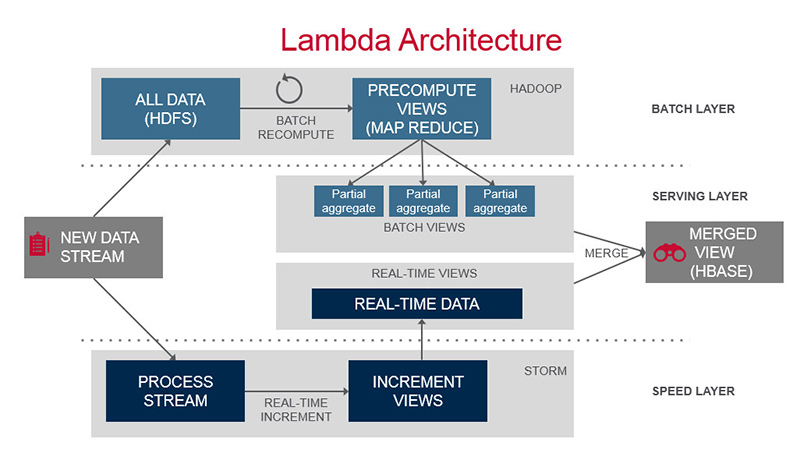
\includegraphics[width=1.0\linewidth]{images/lambda-architecture}
	\caption{Aufbau der Lambda-Architektur} %Generelle
	\label{fig:cnn_structure}
\end{figure}